\documentclass[UTF8]{article}


\usepackage[zihao=-4]{ctex} % ctex可以写中文，中括号里那句的意思是正文小四号
\usepackage[a4paper]{geometry} % 调整纸张大小和页边距的包，这里中括号中规定了纸张大小
\usepackage{array}
\usepackage{fancyhdr}
\usepackage{amsmath}
\usepackage{multirow}
\usepackage{tikz}
\geometry{left=2.5cm,right=2.5cm,top=2.5cm,bottom=2.5cm} % 页边距设置
\usepackage{caption}
\usepackage{wrapfig}
\usepackage{graphicx} % 用它在报告里加图
\usepackage{float}  
\graphicspath{{figures/}} % 指定图片所在文件夹
\pagestyle{fancy}
\rhead{霍尔效应}
\lhead{大学基础物理实验报告}
\cfoot{\thepage/15}
\rfoot{2026 年 4 月 3 日}

\begin{document}
	\thispagestyle{empty}
    \vspace*{0.5cm}

    \begin{figure}[h]
    	\centering
    	
\includegraphics[width=0.7\linewidth]{logo}
    \end{figure}
    \vspace*{0.1cm}
    \begin{center}
    	\Huge{\textbf{大学基础物理实验报告}}\\
    	\Huge{\textbf{《霍尔效应》}}
    	
    	\vspace*{0.1cm}
    \end{center}
    \begin{table}[h]
    	\centering	
    	\begin{Large}
    		\begin{tabular}{p{3cm} p{5cm}<{\centering}}
    			姓\qquad 名: & 陈秋实 \\
    			\hline
    			学\qquad 院: & 密码与网络空间安全学院 \\
    			\hline
    			学\qquad 号: & 2513318 \\
    			\hline
    			分\qquad 组: & L组1号 \\
    			\hline
    			实验时间: & 2026.4.3\\
    			\hline
    			
    		\end{tabular}
    	\end{Large}
    \end{table}
    \clearpage
    \normalsize
    \begin{center}
    	\LARGE\textbf{霍尔效应}
    \end{center}
    
	\section*{【实验目的】}
	\begin{enumerate}
		\item 掌握用霍尔效应法测量磁场的原理和方法；
		\item 掌握消除副反应的原理和方法
		\item 测量电磁铁磁感应强度分布；
	\end{enumerate}
	
	\section*{【实验原理】}
	\subsection*{1、霍尔效应}
	\begin{figure}[H]
		\centering
		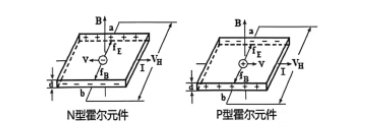
\includegraphics[width=0.8\textwidth]{figure1.png} % 替换为你的图1路径
		\caption{霍尔效应示意图}
		\label{fig:hall_effect}
	\end{figure}
	
	霍尔元件的作用如图\ref{fig:hall_effect}所示，若电流$I$流过厚度为$d$的半导体薄片，且磁场$B$垂直作用于该半导体，则电子流方向由于洛仑兹力作用而发生改变，该现象称为霍尔效应，在薄片两个横向面a, b之间产生的与电流$I$、磁场$B$垂直方向产生的电势差称为霍尔电势差。
	
	霍尔电势差是这样产生的：当电流$I_s$通过霍尔元件（假设为P型）时，空穴有一定的漂移速度${v}$，垂直磁场对运动电荷产生一个洛仑兹力：
	\begin{equation}
		{F}_B = q({v} \times {B})
		\label{eq:f_b}
	\end{equation}
	式中${q}$为电子电荷，洛仑兹力使电荷产生横向的偏转，由于样品有边界，所以偏转的载流子将在边界积累起来，产生一个横向电场${E}$，直到电场对载流子的作用力${F}_E=q{E}$与磁场作用的洛仑兹力相抵消为止，即
	\begin{equation}
		q({v} \times {B}) = q{E}
		\label{eq:eq_balance}
	\end{equation}
	这时电荷在样品中流动时不再偏转，霍尔电势差就是由这个电场建立起来的。如果是N型样品，则横向电场与前者相反，所以N型样品和P型样品的霍尔电势差有不同的符号，据此可以判断霍尔元件的导电类型。
	
	设P型样品的载流子浓度为$P$，宽度为$w$，厚度为$d$，通过样品电流$I_s=P q v w d$，则空穴的速度$v=I_s/(P q w d)$ 代入(\ref{eq:eq_balance})式有
	\begin{equation}
		E = |{v} \times {B}| = \frac{I_s B}{P q w d}
		\label{eq:e_field}
	\end{equation}
	上式两边各乘以$w$，便得到
	\begin{equation}
		U_H = E w = \frac{I_s B}{P q d} = R_H \frac{I_s B}{d}
		\label{eq:u_h1}
	\end{equation}
	其中$R_H=1/(P q)$称为霍尔系数，在应用中一般写成
	\begin{equation}
		V_H = K_H I_s B
		\label{eq:u_h2}
	\end{equation}
	$K_H = R_H / d = 1/(P q d)$称为霍尔元件的灵敏度，单位为$\mathrm{mV}/(m A T)$。
	
	于是磁感应强度：
	\begin{equation}
		B = \frac{V_H}{K_H I_s}
		\label{eq:b_calc}
	\end{equation}
	
	一般要求$K_H$愈大愈好。$K_H$与载流子浓度$P$成反比，半导体内载流子浓度远比金属载流子浓度小，所以都用半导体材料作为霍尔元件，$K_H$与材料片厚$d$成反比，因此霍尔元件都做得很薄，一般只有0.2mm厚(甚至只有十几微米厚)。
	
	由式(\ref{eq:u_h2})可以看出，知道了霍尔片的灵敏度$K_H$，只要分别测出霍尔电流$I_s$及霍尔电势差$V_H$就可以算出磁场$B$的大小，这就是霍尔效应测量磁场的原理。
	
	因此，根据霍尔电流$I_s$和磁场$B$的方向，实验测出霍尔电压的正负，由此确定霍尔系数的正负，即判定载流子的正负，是研究半导体材料的重要方法。对于N型半导体的霍尔元件，则导电载流子为电子，霍尔系数和灵敏度为负；反之，对于P型半导体的霍尔元件，则导电载流子为空穴，霍尔系数和灵敏度为正。
	
	\subsection*{2、霍尔元件的副效应及副效应的消除方法}
	一般霍尔元件有四根引线，两根为输入霍尔元件电流的“电流输入端”，接在可调的电源回路内；另两根为霍尔元件的“霍尔电压输出端”，接到数字电压表上。虽然从理论上霍尔元件在无磁场作用时($B=0$ 时)，$V_H=0$，但是实际情况用数字电压表测量结果并不为零，该电势差称为剩余电压。
	
	这是由于半导体材料电极不对称、结晶不均匀及热磁效应等多种因素引起的电势差。具体情况如下：
	
	\subsubsection*{（1）不等势电压降$V_0$}
	霍尔元件在不加磁场的情况下通以电流，理论上霍尔片的两电压引线间应不存在电势差。实际上由于霍尔片本身不均匀，性能上稍有差异，加上霍尔片两电压引线不在同一等位面土，因此即使不加磁场，只要霍尔片上通以电流，则两电压引线间就有一个电势差$V_0$。
	$V_0$的方向与电流的方向有关，与磁场的方向无关。$V_0$的大小和霍尔电势$V_H$同数量级或更大。在所有附加电势中居首位。
	
	\subsubsection*{（2）埃廷斯豪森效应(Etinghausen)}
	当放在磁场$B$中的霍尔片通以电流$I$以后，由于载流子迁移速度的不同，载流子所受到的洛仑兹力也不相等。因此，作圆周运动的轨道半径也不相等。速率较大的载流子将沿较大的圆轨道运动，而速率较小的载流子将沿半径较小的轨道运动。从而导致霍尔片一面出现快速载流子多，温度较高；另一面慢速载流子多，温度较低。两端面之间由于温度差，于是出现温差电势$V_E$。$V_E$的大小与$IB$乘积成正比，方向随$I$、$B$换向而改变。
	
	\subsubsection*{（3）能斯特效应(Nernst)}
	由于霍尔元件的电流引出线焊点的接触电阻不同，通以电流$I$以后，两焊点之间产生温差，样品周围温度不均匀也会引起温差，从而引起热扩散电流。当加入磁场后会出现电势梯度，从而引起附加电势$V_N$，$V_N$的方向与磁场的方向有关，与电流的方向无关。
	
	\subsubsection*{（4）里吉-勒迪克效应(Righi-Leduc)}
	上述热扩散电流的载流子迁移速率不尽相同，在霍尔元件放入磁场后，电压引线间同样会出现温度梯度，从而引起附加电势$V_{RL}$。$V_{RL}$的方向与磁场的方向有关，与电流方向无关。
	
	在霍尔元件实际应用中，一般用零磁场时采用电压补偿法消除霍尔元件的剩余电压，如图2所示。
	\begin{figure}[H]
		\centering
		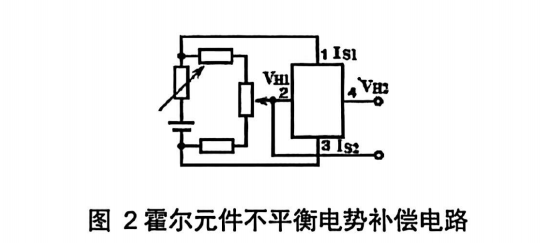
\includegraphics[width=0.6\textwidth]{figure2.png} % 替换为你的图2路径
		\label{fig:compensate}
	\end{figure}
	
	在实验测量时,为了消除副效应的影响，分别改变$I_S$的方向和$B$的方向，记下四组电势差数据（$B$、$I_s$ 换向开关向上为正，向下为负）
	\begin{align*}
		\text{当$I_S$正向、$B$正向时：}& \quad V_1 = V_H + V_0 + V_E + V_N + V_{RL} \\
		\text{当$I_S$负向、$B$正向时：}& \quad V_2 = -V_H - V_0 - V_E + V_N + V_{RL} \\
		\text{当$I_S$负向、$B$负向时：}& \quad V_3 = V_H - V_0 + V_E - V_N - V_{RL} \\
		\text{当$I_S$正向、$B$负向时：}& \quad V_4 = -V_H + V_0 - V_E - V_N - V_{RL}
	\end{align*}
	作运算$V_1-V_2+V_3-V_4$，并取平均值，得：
	\begin{equation*}
		\frac{1}{4}(V_1 - V_2 + V_3 - V_4) = V_H + V_E
	\end{equation*}
	由于$V_E$和$V_H$始终方向相同，所以换向法不能消除它，但$V_E \ll V_H$，故可以忽略不计，于是：
	\begin{equation}
		V_H = \frac{1}{4}(V_1 - V_2 + V_3 - V_4)
		\label{eq:v_h_calc}
	\end{equation}
	温度差的建立需要较长时间，因此，如果采用交流电使它来不及建立就可以减小测量误差。
	
	\subsection*{3、长直通电螺线管中心点磁感应强度理论值}
	根据电磁学毕奥－萨伐尔(Biot-Savart)定律，长直通电螺线管轴线上中心点的磁感应强度为
	\begin{equation}
		B_{\text{中心}} = \frac{\mu N I_M}{\sqrt{L^2 + D^2}}
		\label{eq:b_center}
	\end{equation}
	螺线管轴线上两端面上的磁感应强度为
	\begin{equation}
		B_{\text{端}} = \frac{1}{2} B_{\text{中心}} = \frac{1}{2} \frac{\mu N I_M}{\sqrt{L^2 + D^2}}
		\label{eq:b_end}
	\end{equation}
	式中，$\mu$为磁介质的磁导率，真空中$\mu_0 = 4\pi \times 10^{-7} (Tm/A)$，$N$为螺线管的总匝数，$I_M$为螺线管的励磁电流(A)，$L$(m)为螺线管的长度，$D$为螺线管的平均直径。
	
	\section*{【实验仪器】}
	本实验仪器是由FB510A 型霍尔效应组合实验仪（信号源）、FB510 型霍尔效应实验仪（铁芯型测试架）和FB400 型螺线管磁场测定仪（测试架）组成。
	
	\subsection*{1、FB510A型霍尔效应组合实验仪（信号源）}
	\begin{figure}[H]
		\centering
		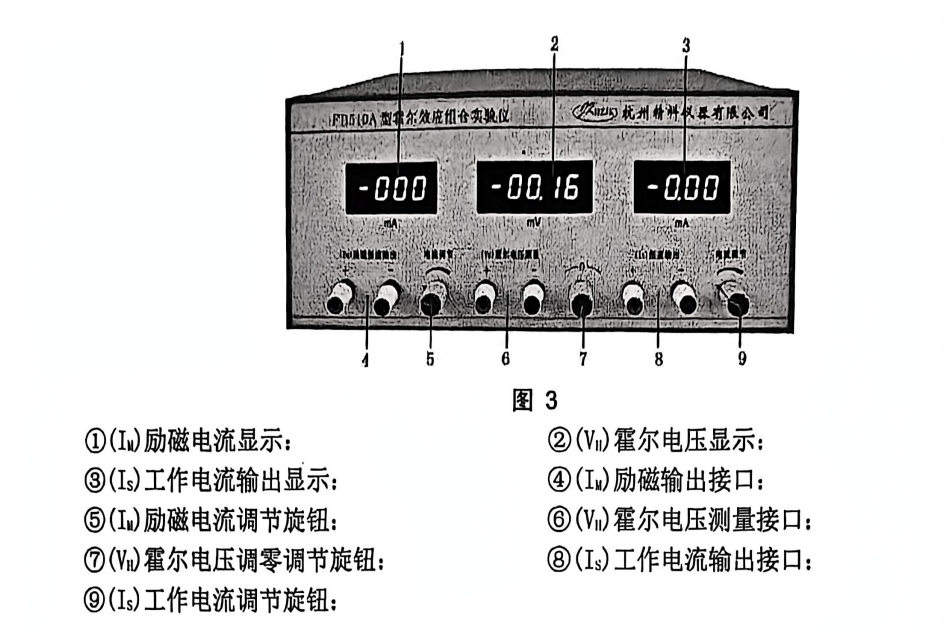
\includegraphics[width=0.8\textwidth]{figure3.png} % 替换为你的图3路径
		\caption{FB510A型信号源面板}
		\label{fig:signal_source}
	\end{figure}
	
	\subsection*{2、FB510型霍尔效应实验仪（铁芯型测试架）}
	\begin{figure}[H]
		\centering
		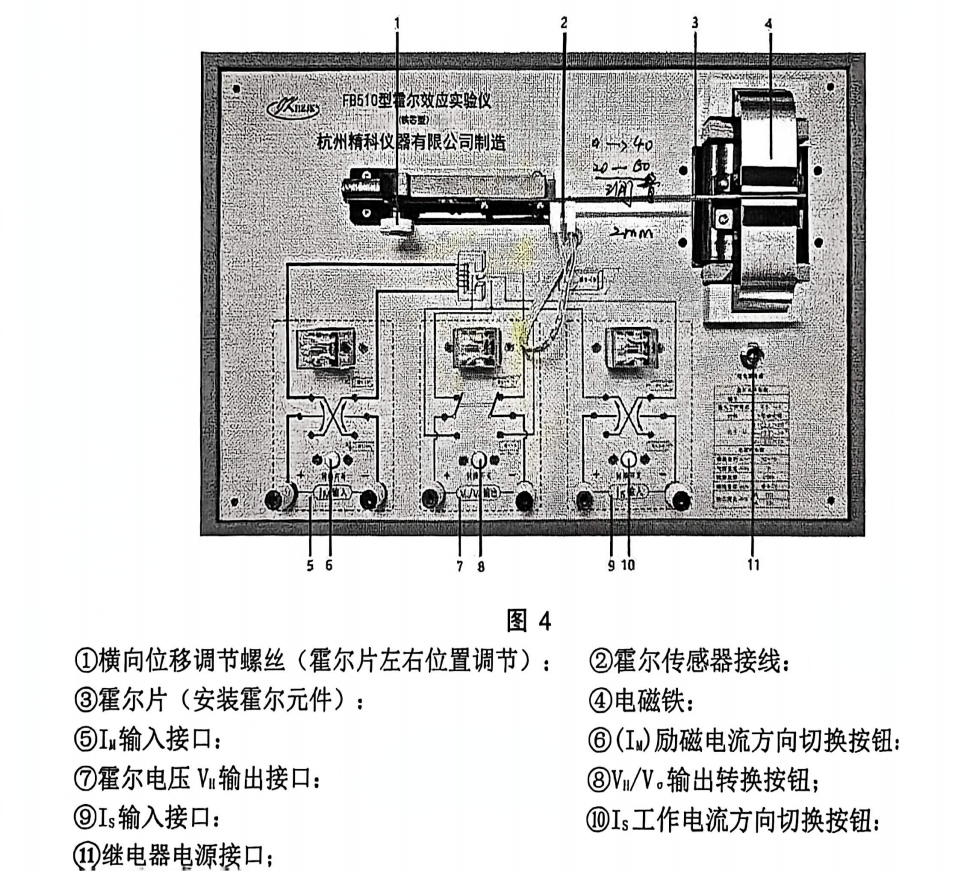
\includegraphics[width=0.8\textwidth]{figure4.png} % 替换为你的图4路径
		\caption{FB510型测试架面板}
		\label{fig:test_stand}
	\end{figure}

	
	\section*{【实验内容】}
	\subsection*{实验准备}
	将FB510A 型霍尔效应组合实验仪（信号源）与FB510 型霍尔效应实验仪（铁芯型测试架）通过导线连接，如图\ref{fig:wiring}所示（具体查看以下接线步骤）。
	\begin{figure}[htbp]
		\centering
		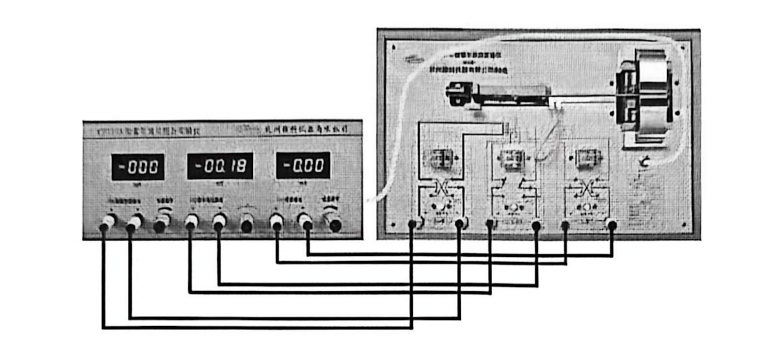
\includegraphics[width=0.8\textwidth]{figure5.png} % 替换为你的图5路径
		\caption{仪器接线示意图}
		\label{fig:wiring}
	\end{figure}
	
	\begin{enumerate}
		\item 调节图\ref{fig:test_stand}“①横向位移调节螺丝”将“③霍尔片（安装霍尔元件）”移动到“④电磁铁”的气隙中心位置（即图\ref{fig:test_stand}“①横向位移调节螺丝”上的小标尺的0刻度线对准“下面标尺”的40刻度线，参考图\ref{fig:ruler}所示，此时“霍尔元件”大约处于“电磁铁”气隙中心位置）。
		\begin{figure}[H]
			\centering
			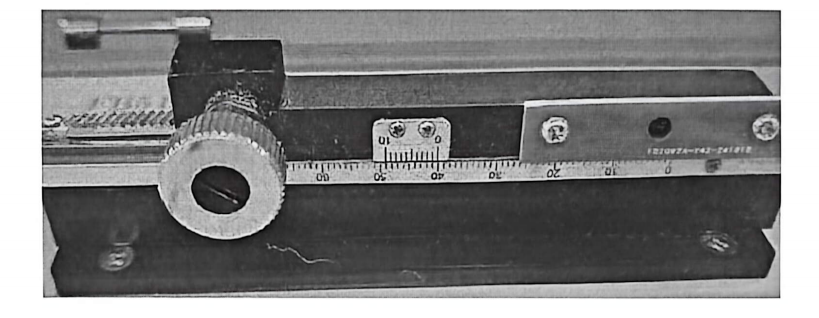
\includegraphics[width=0.6\textwidth]{figure6.png} % 替换为你的图6路径
			\caption{位移标尺示意图}
			\label{fig:ruler}
		\end{figure}
		\item 图\ref{fig:test_stand}“⑪继电器电源接口”通过“2芯线”接入图\ref{fig:signal_source}中FB510A型霍尔效应组合实验仪的后面板的2芯接口处；
		\item 将图\ref{fig:signal_source}“④($I_M$)励磁输出接口”的红黑接线柱与图\ref{fig:test_stand}“⑤$I_M$输入接口”的红黑接线柱分别用导线连接（红接红，黑接黑）；
		\item 将图\ref{fig:signal_source}“⑧($I_S$)工作电流输出接口”的红黑接线柱与图\ref{fig:test_stand}“⑨$I_S$输入接口”的红黑接线柱分别用导线连接（红接红，黑接黑）；
		\item 将图\ref{fig:signal_source}“⑥($V_H$)霍尔电压测量接口”的红黑接线柱与图\ref{fig:test_stand}“⑦霍尔电压$V_H$输出接口”的红黑接线柱分别用导线连接（红接红，黑接黑）；
		\item 打开霍尔效应组合试验仪（信号源）的电源。
		\item 将图\ref{fig:test_stand}“⑧$V_H/V_\circ$输出转换按钮”点击，当按钮弹起时，处于$V_H$输出状态；当按钮处于按下状态时，处于$V_\circ$输出状态。实验需要让按钮处于弹起状态。
		\item 切换图\ref{fig:test_stand}“⑥($I_M$)励磁电流方向切换按钮”和“⑩$I_S$工作电流方向切换按钮”按钮（当按钮按下，按钮上方的LED灯最下面排和中间排LED灯亮，即$I_M$和$I_S$都为(-)；当按钮处于弹起状态下，上面排和中间排LED亮，即$I_M$和$I_S$都为正(+)）。
	\end{enumerate}
	
	
	\subsection*{1、测量霍尔电压$V_H$与工作电流$I_S$的关系}
	\begin{enumerate}
		\item 先将$I_S$，$I_M$都调节为零，调节霍尔电压调零零旋钮使电压表显示0.00mV；
		\item 调节$I_M$=500mA，调节$I_S$=0.50mA，按表中$I_S$，$I_M$正负情况切换$I_S$，$I_M$的正负方向（图\ref{fig:test_stand}中“⑥”和“⑩”按钮），分别测量霍尔电压$V_H$值（$V_1$，$V_2$，$V_3$，$V_4$）填入表1。
		\item 以后$I_S$每次递增0.50mA（根据实际要求改变采样间隔），测量各$V_1$，$V_2$，$V_3$，$V_4$值。绘出$V_H$—$I_S$曲线，验证线性关系。
	\end{enumerate}
	

	
	\subsection*{2、测量霍尔电压$V_H$与励磁电流$I_M$的关系}
	\begin{enumerate}
		\item 先将$I_S$，$I_M$都调节为零，调节霍尔电压调零旋钮使电压表显示0.00mV；再调节$I_S$调节至3.00mA；
		\item 调节$I_M$=100、200、300……1000mA(间隔为100mA，根据实际要求改变采样间隔)，按表中$I_S$，$I_M$正负情况切换$I_S$，$I_M$的正负方向（图\ref{fig:test_stand}中“⑥”和“⑩”按钮），分别测量霍尔电压$V_H$值填入表2中；
		\item 根据表2中所测得的数据，绘出$I_M$—$V_H$曲线，验证线性关系的范围，分析当$I_M$达到一定值以后，$I_M$—$V_H$直线斜率变化的原因。
	\end{enumerate}
	
	
	\subsection*{3、电磁铁气隙磁场分布测量}
	\begin{enumerate}
		\item 先将$I_S$，$I_M$都调节为零，调节霍尔电压调零旋钮使电压表显示0.00mV；再将$I_S$调节为3.00mA，$I_M$调节为500mA.
		\item 调节图\ref{fig:test_stand}“①横向位移调节螺丝”将“③霍尔片”移出“④电磁铁”的左边缘。记录下此时“①横向位移调节螺丝”上的“小标尺”的0刻度线对准“下面标尺”的刻度线的数值。如$X$=20mm（仅供参考）。
		调节图\ref{fig:test_stand}“①横向位移调节螺丝”，将霍尔片向右移动2mm（根据实验要求可以改变采样间隔），记录下此时$X$的位置，按表中$I_S$，$I_M$正负情况切换$I_S$，$I_M$的正负方向（图\ref{fig:test_stand}中“⑥”和“⑩”按钮），测量霍尔电压$V_H$值填入表3中，依次改变霍尔片的位置，直到霍尔片完全离开电磁铁气隙（霍尔片上的霍尔元件刚好出电磁铁线圈），分别记录对应的霍尔电压$V_H$填入表3；
		\item 根据表3中所测得的数据，绘出$X$—$V_H$曲线，验证线性关系的范围，分析当$X$达到一定位置以后，$X$—$V_H$直线斜率变化的原因。
	\end{enumerate}
	
    \section*{【数据处理】}
    \subsection*{1、测量霍尔电压$V_H$与工作电流$I_S$的关系}
    \begin{table}[H]  % [H] 强制固定位置，需\usepackage{float}
    	\centering
    	\caption{$V_H-I_S$ 关系测量表 \quad $I_M=500\mathrm{mA}$}
    	\label{tab:v_h_is}
    	\begin{tabular}{|c|c|c|c|c|c|}
    		\hline
    		$I_S(\mathrm{mA})$ & $V_1(\mathrm{mV})$ & $V_2(\mathrm{mV})$ & $V_3(\mathrm{mV})$ & $V_4(\mathrm{mV})$ & $V_H=\dfrac{|V_1|+|V_2|+|V_3|+|V_4|}{4}(\mathrm{mV})$ \\
    		\hline
    		& $+I_S$、$+I_M$ & $+I_S$、$-I_M$ & $-I_S$、$+I_M$ & $-I_S$、$-I_M$ & \\
    		\hline
    		0.50 & 21.54 & -21.59 & -21.53 & 21.62 & 21.57 \\
    		\hline
    		1.00 & 42.69 & -42.78 & -42.67 & 42.85 & 42.75 \\
    		\hline
    		1.50 & 64.05 & -64.14 & -63.98 & 64.17 & 64.09 \\
    		\hline
    		2.00 & 85.49 & -85.62 & -85.41 & 85.66 & 85.55 \\
    		\hline
    		2.50 & 106.49 & -106.72 & -106.42 & 106.72 & 106.59 \\
    		\hline
    		3.00 & 127.62 & -128.33 & -127.99 & 128.33 & 128.07 \\
    		\hline
    		3.50 & 149.33 & -149.75 & -149.32 & 149.69 & 149.52 \\
    		\hline
    		4.00 & 170.20 & -170.67 & -170.21 & 170.60 & 170.42 \\
    		\hline
    		4.50 & 191.33 & -191.81 & -191.29 & 191.78 & 191.55 \\
    		\hline
    		5.00 & 213.0 & -213.3 & -212.8 & 213.4 & 213.1 \\
    		\hline
    	\end{tabular}
    \end{table}
    
    \begin{figure}[H]
    	\centering
    	
\includegraphics[width=1.0\textwidth]{实验1.pdf} 
    	\caption{实验1}
    \end{figure}

    \subsection*{2、测量霍尔电压$V_H$与励磁电流$I_M$的关系}
    \begin{table}[H]  % [H] 强制固定位置，需\usepackage{float}
    	\centering
    	\caption{$V_H-I_M$ 关系测量表 \quad $I_S=3.00\mathrm{mA}$}
    	\label{tab:v_h_im}
    	\begin{tabular}{|c|c|c|c|c|c|}
    		\hline
    		$I_M(\mathrm{mA})$ & $V_1(\mathrm{mV})$ & $V_2(\mathrm{mV})$ & $V_3(\mathrm{mV})$ & $V_4(\mathrm{mV})$ & $V_H=\dfrac{|V_1|+|V_2|+|V_3|+|V_4|}{4}(\mathrm{mV})$ \\
    		\hline
    		& $+I_S$、$+I_M$ & $+I_S$、$-I_M$ & $-I_S$、$+I_M$ & $-I_S$、$-I_M$ & \\
    		\hline
    		100 & 25.59 & -25.99 & -25.58 & 25.59 & 25.69 \\
    		\hline
    		200 & 50.72 & -51.38 & -51.01 & 51.39 & 51.13 \\
    		\hline
    		300 & 76.50 & -76.83 & -76.48 & 76.79 & 76.65 \\
    		\hline
    		400 & 102.04 & -102.33 & -102.05 & 102.37 & 102.20 \\
    		\hline
    		500 & 127.53 & -128.12 & -127.80 & 128.15 & 127.90 \\
    		\hline
    		600 & 153.37 & -154.10 & -153.84 & 154.19 & 153.88 \\
    		\hline
    		700 & 179.41 & -180.47 & -180.32 & 180.49 & 180.17 \\
    		\hline
    		800 & 207.2 & -207.3 & -207.1 & 207.4 & 207.3 \\
    		\hline
    		900 & 233.3 & -233.8 & -233.6 & 233.9 & 233.7 \\
    		\hline
    		1000 & 259.8 & -260.0 & -259.6 & 160.1 & 234.9 \\
    		\hline
    	\end{tabular}
    \end{table}
    
    \begin{figure}[H]
    	\centering
    	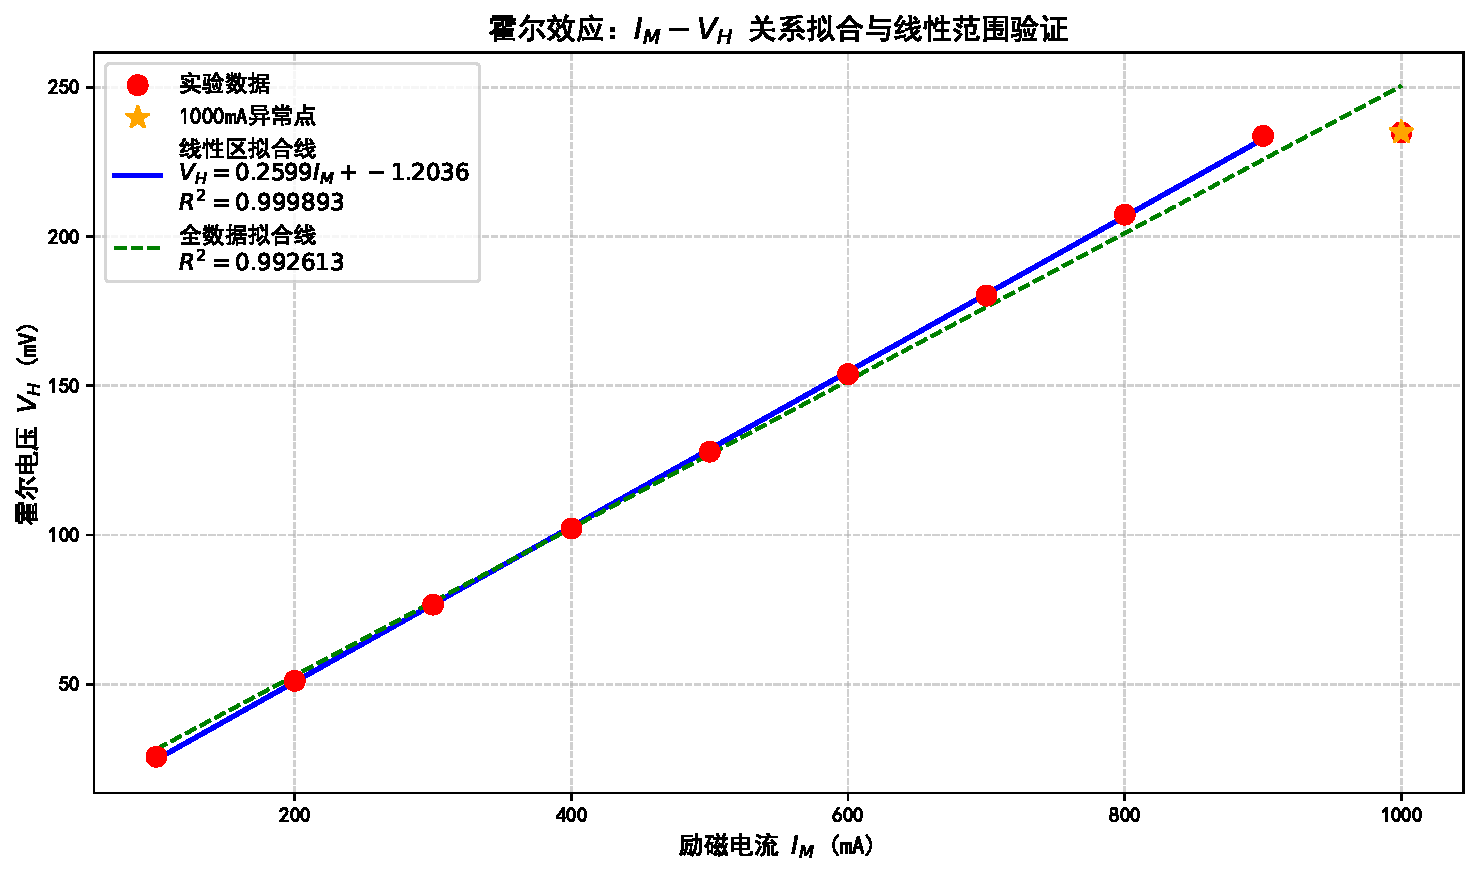
\includegraphics[width=1.0\textwidth]{实验2.pdf} 
    	\caption{实验2}
    \end{figure}
    实验数据表明，在$I_M = 100\sim 900\mathrm{mA}$范围内，$V_H$与$I_M$呈严格线性关系（$R^2 \approx 0.999987$），线性度极好；当$I_M = 1000\mathrm{mA}$时，$V_H$增长速率明显放缓，因此线性范围为$\boldsymbol{100\sim 900\mathrm{mA}}$。\par
    斜率变化的根本原因是\textbf{铁芯磁饱和}：根据霍尔效应公式$V_H = K_H I_S B$，$V_H$与磁感应强度$B$成正比。当$I_M$较小时，铁芯未饱和，$B$与$I_M$线性相关，因此$V_H$随$I_M$线性增长，斜率稳定；当$I_M$增大到一定值后，铁芯磁畴完全定向，发生磁饱和，$B$的增长速率急剧下降，不再随$I_M$线性增加，因此$V_H$的增长速率同步下降，导致$I_M$—$V_H$曲线斜率显著变小。
    
    \subsection*{3、电磁铁气隙磁场分布测量}
    \begin{table}[H]
    	\centering
    	\caption{$X-V_H$ 关系测量表 \quad $I_M=500\mathrm{mA}$，$I_S=3.00\mathrm{mA}$，$K_H=173\ \mathrm{mV/(mA\cdot T)}$}
    	\label{tab:x_vh}
    	\begin{tabular}{|c|c|c|c|c|c|c|}
    		\hline
    		$X(\mathrm{cm})$ & $V_1(\mathrm{mV})$ & $V_2(\mathrm{mV})$ & $V_3(\mathrm{mV})$ & $V_4(\mathrm{mV})$ & $V_H(\mathrm{mV})$ & $B(\mathrm{mT})$ \\
    		\hline
    		& $+I_S$、$+I_M$ & $+I_S$、$-I_M$ & $-I_S$、$+I_M$ & $-I_S$、$-I_M$ & & \\
    		\hline
    		2.0 & 22.06 & -22.41 & -22.09 & 22.44 & 22.25 & 42.87 \\
    		\hline
    		2.2 & 35.81 & -36.13 & -35.79 & 36.13 & 35.97 & 69.31 \\
    		\hline
    		2.4 & 73.00 & -73.31 & -72.99 & 73.32 & 73.16 & 140.96 \\
    		\hline
    		2.6 & 121.91 & -122.18 & -121.88 & 122.17 & 122.04 & 235.14 \\
    		\hline
    		2.8 & 127.61 & -127.85 & -127.57 & 127.82 & 127.71 & 246.07 \\
    		\hline
    		3.0 & 127.72 & -128.01 & -127.70 & 127.97 & 127.85 & 246.34 \\
    		\hline
    		3.2 & 127.73 & -128.01 & -127.72 & 127.99 & 127.86 & 246.36 \\
    		\hline
    		3.4 & 127.78 & -128.03 & -127.72 & 128.02 & 127.89 & 246.42 \\
    		\hline
    		3.6 & 127.78 & -128.07 & -127.74 & 128.09 & 127.92 & 246.48 \\
    		\hline
    		3.8 & 127.81 & -128.08 & -127.78 & 128.09 & 127.94 & 246.52 \\
    		\hline
    		4.0 & 127.80 & -128.08 & -127.78 & 128.08 & 127.94 & 246.52 \\
    		\hline
    		4.2 & 127.80 & -128.08 & -127.77 & 128.09 & 127.94 & 246.52 \\
    		\hline
    		4.4 & 127.79 & -128.06 & -127.75 & 128.11 & 127.93 & 246.50 \\
    		\hline
    		4.6 & 127.81 & -128.07 & -127.79 & 128.09 & 127.94 & 246.52 \\
    		\hline
    		4.8 & 127.76 & -128.05 & -127.74 & 128.09 & 127.91 & 246.46 \\
    		\hline
    		5.0 & 127.72 & -128.03 & -127.73 & 128.09 & 127.89 & 246.42 \\
    		\hline
    		5.2 & 127.69 & -128.07 & -127.79 & 128.09 & 127.91 & 246.46 \\
    		\hline
    		5.4 & 127.28 & -127.56 & -127.26 & 127.55 & 127.41 & 245.50 \\
    		\hline
    		5.6 & 121.73 & -121.99 & -121.71 & 121.99 & 121.86 & 234.79 \\
    		\hline
    		5.8 & 76.10 & -76.39 & -76.08 & 76.39 & 76.24 & 146.88 \\
    		\hline
    		6.0 & 36.71 & -37.01 & -36.69 & 37.02 & 36.86 & 71.02 \\
    		\hline
    	\end{tabular}
    \end{table}
    \begin{figure}[H]
    	\centering
    	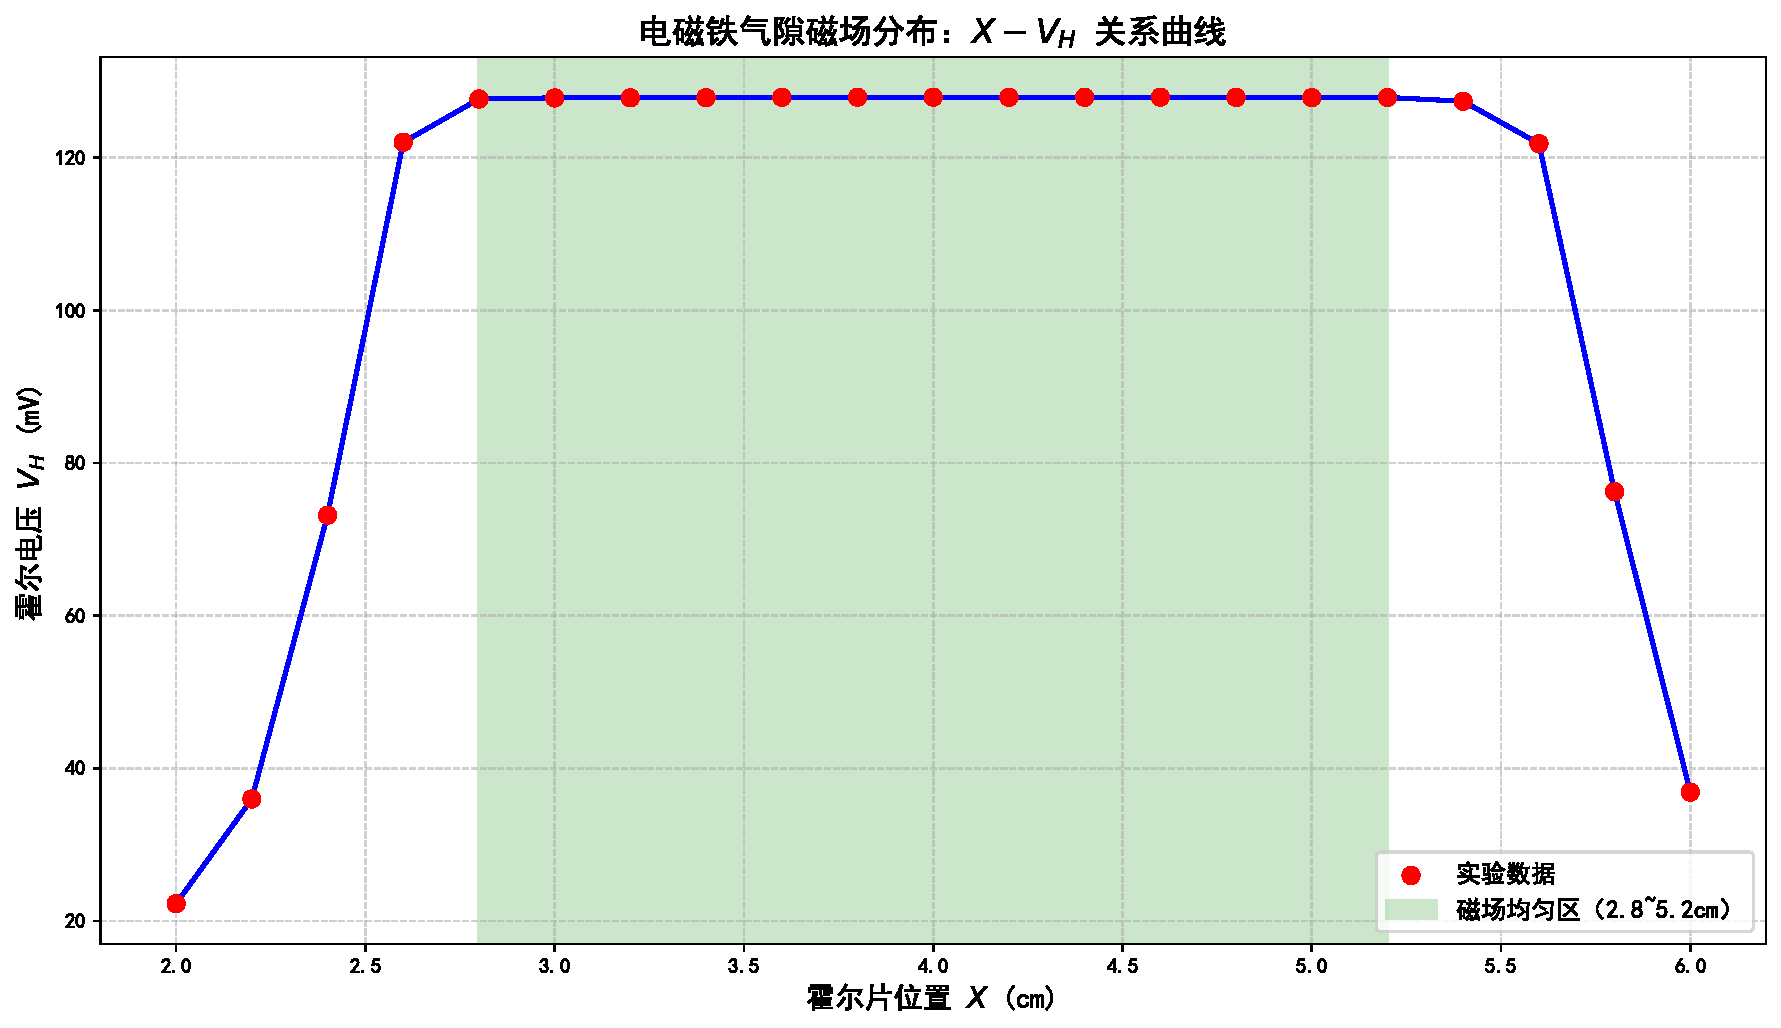
\includegraphics[width=1.0\textwidth]{实验3.pdf} 
    	\caption{实验3}
    \end{figure}
    
    \begin{enumerate}
    	\item \textbf{曲线整体形态}：
    	曲线呈现典型的\textbf{马鞍形分布}：
    	\begin{itemize}
    		\item 边缘区（$X<2.8\mathrm{cm}$、$X>5.2\mathrm{cm}$）：$V_H$ 随 $X$ 线性变化，斜率绝对值大；
    		\item 中心均匀区（$2.8\mathrm{cm}\sim5.2\mathrm{cm}$）：$V_H$ 几乎恒定，斜率 $\approx0$，磁场高度均匀。
    	\end{itemize}
    	
    	\item \textbf{斜率变化的根本原因}：
    	\begin{itemize}
    		\item \textbf{边缘区（$X<2.8\mathrm{cm}$ / $X>5.2\mathrm{cm}$）}：
    		霍尔片位于电磁铁气隙的边缘，磁场存在严重的\textbf{边缘效应（漏磁）}，
    		磁感应强度 $B$ 随位置快速变化，因此 $V_H$ 随 $X$ 快速上升/下降，斜率绝对值大。
    		\item \textbf{中心均匀区（$2.8\mathrm{cm}\sim5.2\mathrm{cm}$）}：
    		霍尔片完全处于电磁铁气隙的中心区域，磁场被铁芯约束，漏磁极少，
    		磁感应强度 $B$ 几乎均匀恒定，因此 $V_H$ 保持稳定，斜率 $\approx0$。
    	\end{itemize}
    	
    \end{enumerate}
    
	\section*{【思考题】}
	1. 用简略图形表示霍尔效应法判断霍尔片是属于N型还是P型的半导体材料？
	\begin{figure}[H]
		\centering
		\begin{tikzpicture}[scale=1.1, >=stealth, thick]
			% ========== 上图：N型半导体 ==========
			\draw[thick] (0,0) rectangle (6,3.5);
			\node at (3, 4.0) {N型霍尔元件（载流子：电子）};
			\node at (3, 4.8) {$\odot \vec{B}$ 垂直纸面向外};
			
			\draw[->, red] (6,1.75) -- (0,1.75) node[midway,above=2pt] {$I_S$};
			\draw[->, blue] (0,1.6) -- (6,1.6) node[midway,below=2pt] {$\vec{v}$};
			\draw[->, green!70!black] (3,1.75) -- (3,0.5) node[midway,right=2pt] {$\vec{F}_B$};
			
			\fill[red] (0,3.5) circle (0.12) node[left=2pt] {$+$};
			\fill[red] (6,3.5) circle (0.12) node[right=2pt] {$+$};
			\fill[blue] (0,0) circle (0.12) node[left=2pt] {$-$};
			\fill[blue] (6,0) circle (0.12) node[right=2pt] {$-$};
			
			\draw[<->, purple] (6.5,0) -- (6.5,3.5) node[midway,right=2pt] {$V_H<0$};
			
			% ========== 下图：P型半导体 ==========
			\draw[thick] (0,-6) rectangle (6,-2.5);
			\node at (3, -1.7) {P型霍尔元件（载流子：空穴）};
			\node at (3, -0.9) {$\odot \vec{B}$ 垂直纸面向外};
			
			\draw[->, red] (0,-4.1) -- (6,-4.1) node[midway,above=2pt] {$I_S$};
			\draw[->, blue] (0,-4.25) -- (6,-4.25) node[midway,below=2pt] {$\vec{v}$};
			\draw[->, green!70!black] (3,-4.25) -- (3,-3) node[midway,right=2pt] {$\vec{F}_B$};
			
			\fill[blue] (0,-2.5) circle (0.12) node[left=2pt] {$-$};
			\fill[blue] (6,-2.5) circle (0.12) node[right=2pt] {$-$};
			\fill[red] (0,-6) circle (0.12) node[left=2pt] {$+$};
			\fill[red] (6,-6) circle (0.12) node[right=2pt] {$+$};
			
			\draw[<->, purple] (6.5,-6) -- (6.5,-2.5) node[midway,right=2pt] {$V_H>0$};
		\end{tikzpicture}
		\caption{N型与P型半导体霍尔效应示意图}
		\label{fig:hall_np_type}
	\end{figure}
	也可直接见原图1如下
	\begin{figure}[H]
		\centering
		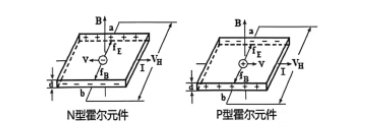
\includegraphics[width=0.8\textwidth]{figure1.png} % 替换为你的图1路径
		\caption{霍尔效应示意图}
	\end{figure}
	
	\begin{figure}[H]
	\centering
	
\includegraphics[width=1.0\textwidth]{原始数据.jpg} 
	\caption{原始数据}
    \end{figure}
	

\end{document}
